% ============================================================
%  CHAPITRE 1 — LES BASES
% ============================================================
\chapter{Les Bases}

\chapintro{Ce chapitre présente le contexte général du projet \textbf{MecaRage}~:
la structure de l'entreprise commanditaire, la problématique à l'origine du projet
et la solution proposée.}

\section{Introduction}

Dans un contexte de digitalisation croissante des métiers de la maintenance
automobile, les ateliers mécaniques ressentent une pression de plus en plus forte
pour moderniser leurs processus. MecaRage a été conçu pour répondre à ce besoin
en offrant une solution numérique complète, couvrant l'ensemble de la chaîne
opérationnelle d'un réseau d'ateliers multi-sites.

\section{Présentation de l'entreprise}

L'entreprise partenaire coordonne plusieurs \textit{garages} répartis géographiquement,
chacun disposant d'une équipe de mécaniciens supervisée par un chef d'atelier.
La direction centrale assure la supervision globale des opérations et de la facturation.

\section{Présentation du projet}

\subsection{Problématique}

La gestion d'un réseau d'ateliers mécaniques implique une coordination complexe
entre plusieurs parties prenantes~: les clients qui déposent leurs véhicules,
les mécaniciens qui exécutent les travaux, le chef d'atelier qui orchestre les
ressources, et la direction qui supervise les finances.

\begin{table}[H]
\centering
\caption{Problèmes identifiés dans le système actuel}
\label{tab:problemes}
\begin{tabularx}{\textwidth}{|l|X|X|}
\hline
\rowcolor{gray!20}
\textbf{Domaine} & \textbf{Problème} & \textbf{Conséquence} \\
\hline
Communication & RDV par téléphone/WhatsApp & Pas de traçabilité \\
\hline
Rapports & Fiches papier mécanicien & Risque de perte, illisibilité \\
\hline
Facturation & Tableur Excel par garage & Pas de vision consolidée \\
\hline
Suivi & Aucun outil de statut en temps réel & Manque de visibilité client \\
\hline
Diagnostic & Réception sans pré-analyse & Perte de temps à l'accueil \\
\hline
Stock & Inventaire manuel pièces & Ruptures non anticipées \\
\hline
\end{tabularx}
\end{table}

\subsection{Étude de l'existant}

L'existant se compose d'une combinaison d'outils non intégrés~:

\begin{table}[H]
\centering
\caption{Outils existants et leurs limites}
\label{tab:existant}
\begin{tabularx}{\textwidth}{|l|X|X|}
\hline
\rowcolor{gray!20}
\textbf{Outil} & \textbf{Usage actuel} & \textbf{Limite principale} \\
\hline
WhatsApp / SMS & Prise de RDV, communications & Informel, non traçable \\
\hline
Excel & Inventaire pièces, facturation & Pas de collaboration temps réel \\
\hline
Papier & Rapports mécaniciens & Perte, archivage difficile \\
\hline
Tableau blanc & Suivi visuel de l'atelier & Non numérique, local uniquement \\
\hline
\end{tabularx}
\end{table}

\subsection{Solution proposée}

\textbf{MecaRage} est une plateforme numérique unifiée couvrant l'intégralité du
cycle de vie d'une intervention mécanique.

\begin{figure}[H]
\centering
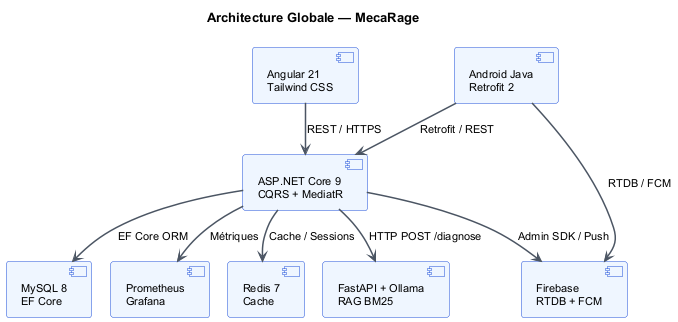
\includegraphics[width=0.82\textwidth]{diagrams/arch_global.png}
\caption{Architecture globale de la plateforme MecaRage}
\label{fig:archi-global}
\end{figure}

\noindent Les apports clés~:
\begin{itemize}[noitemsep]
  \item \textbf{Application web} accessible par tous les rôles (Angular 21).
  \item \textbf{Back-end robuste} (ASP.NET Core 9, Clean Architecture, CQRS).
  \item \textbf{Service IA} (FastAPI + Google Gemini) pour le diagnostic préliminaire.
  \item \textbf{Module mobile Android} (Java) avec Firebase temps réel.
  \item \textbf{Gestion multi-tenant}~: plusieurs entreprises sur la même plateforme.
  \item \textbf{Intervention Lifecycle Tracker}~: suivi automatique sur 10 états.
  \item \textbf{Génération PDF} des factures via QuestPDF.
\end{itemize}

\section{Conclusion}

Ce chapitre a présenté le contexte métier qui a motivé la création de MecaRage.
Le chapitre suivant détaille les spécifications fonctionnelles et techniques.
